\documentclass[a4paper,10pt]{book}
\usepackage{xypic}
\usepackage[centertags]{amsmath}
\usepackage{amscd}
\usepackage{amsthm}
\usepackage{amssymb}
\usepackage{enumerate}
\usepackage{multicol}
\usepackage[english,catalan,spanish]{babel}
\usepackage[all]{xy}
\usepackage{color}
\usepackage{tikz}
\usepackage{indentfirst}
\usepackage[utf8]{inputenc}
\usepackage[T1]{fontenc}
\linespread{1.1}
\setlength{\parskip}{10pt}
\usepackage[twoside,bindingoffset=1cm]{geometry}
\usepackage{lmodern}


%% Custom packages


%%%%%%%%%%%%%%%%%%%%%%%%%%%%%%%%%%%%%%%%%%%%%%%%%%%%%%%%%%%%%%%%%%%%%%%%%%%
%%%% local definitions for this paper
%%%%%%%%%%%%%%%%%%%%%%%%%%%%%%%%%%%%%%%%%%%%%%%%%%%%%%%%%%%%%%%%%%%%%%%%%%%


%%%%%%%%%%%%%%%%%%%%%% aix{\`o} pels headings %%%%%%%%%%%%%%%%%%%%%%%%
\usepackage{fancyhdr}
\pagestyle{fancy}
\renewcommand{\chaptermark}[1]{\markboth{#1}{}}
\renewcommand{\sectionmark}[1]{\markright{\thesection\ #1}}
\fancyhf{} \fancyhead[LE,RO]{\bfseries\thepage}
\fancyhead[LO]{\bfseries\rightmark} \fancyhead[RE]{\bfseries\leftmark}

\def\paginaenblanc{\newpage%
\thispagestyle{empty}%
\vspace*{2cm}%
\newpage%
\thispagestyle{empty}%
}


%%%%%%%%%%%%%%%%%%%%%%%%%%%%%%%%%%%%%%%%%%%%%%%%%%%%%%%%%%%%%%%%%%%%%%%%%
% aux commands
%%%%%%%%%%%%%%%%%%%%%%%%%%%%%%%%%%%%%%%%%%%%%%%%%%%%%%%%%%%%%%%%%%%%%%%%%
%==========================================================================
% macros to support private authors' notes
%==========================================================================
\newif\ifprivate
\privatetrue
\def\xbar{\vskip0.09in\hrule\vskip0.06in}
\def\private#1{\ifprivate \xbar {\em #1} \xbar
\else \fi}
\def\huh{\ifprivate ??? \marginpar{\Huge ???}
\else \fi}
\def\???{\ifprivate {\bf {???}} \marginpar{\begin{center}{\Huge {\bf ?}}\end{center}}
\else \fi}
%\def\???{\ifprivate {\bf {???}} \marginpar{{\Huge {\bf ?}}}
%\else \fi}
\marginparsep1mm
\def\nota#1{\ifprivate  $\clubsuit$ \marginpar{\parbox[t]{2.4cm}{\begin{center}\tiny #1\end{center}}}
\else \fi}
\def\comment#1{\ifprivate \marginpar{\parbox[t]{2.4cm}{\begin{center}\tiny #1\end{center}}}
\else \fi}
%\def\nota#1{\ifprivate  $\clubsuit$ \marginpar{\parbox[t]{1.8cm}{\tiny #1}}
%\else \fi}
\def\privateeject{\ifprivate\eject\fi}
%\def\???{{\bf {???}} \marginpar{{\Huge {\bf ?}}} }
%%%%%%%%%%%%%%%%%%%%%%%%%%%%%%%%%%%%%%%%%%%%%%%%%%%%%%%%%%%%%%%%%%%%%%%%%%

%%%%%%%%%%%%%%%%%%%%%%%%%%%%%%%%%%%%%%%%%%%%%%%%%%%%%%%%%%%%%%%%%%%%%%%%
%%%%%%%%%%%%%%%%%%%%%%%%%%%%%%%%%%%%%%%%%%%%%%%%%%%%%%%%%%%%%%%%%%%%%%%%
\begin{document}

\pagestyle{empty}

\begin{titlepage}
\begin{center}
\begin{figure}[htb]
\begin{center}

\includegraphics[width=6cm]{assets/ub_color.pdf}
\end{center}
\end{figure}

\def\worktitle{Development of an AI-Based Tool for Molecular Subtype Classification of Invasive Ductal Breast Carcinoma Using Mammography}

\textbf{\LARGE Treball final de grau} \\
\vspace*{.5cm}
\textbf{\LARGE GRAU D'ENGINYERIA INFORM\`{A}TICA } \\
\vspace*{.5cm}
\textbf{\LARGE Facultat de Matem\`atiques i Inform\`atica\\ Universitat de Barcelona} \\
\vspace*{1.0cm}
\rule{16cm}{0.1mm}\\
\begin{Huge}
\textbf{Development of an AI-Based Tool for Molecular Subtype Classification of Invasive Ductal Breast Carcinoma Using Mammography} \\
\end{Huge}
\rule{16cm}{0.1mm}\\

\vspace{1cm}

\begin{flushright}


\vspace*{2.5cm}

\hfill

\renewcommand{\arraystretch}{1.5}
\begin{tabular}{ll}
\textbf{\small Autor:} & \textbf{\small David Bland\'on T\'orrez } \\
\textbf{\small Director:} & \textbf{\small Dr. Oliver D\'iaz Montesdeoca } \\
\textbf{\small Realitzat a:} & \textbf{\small  Departament de Matem\`{a}tiques i  Inform\`{a}tica  } \\
\textbf{\small Barcelona,} & \textbf{\small \today }
\end{tabular}

\end{flushright}

\end{center}

\end{titlepage}

%%%%%%%%%%%%%%%%%%%%%%%%%%%%%%%%%%%%%%%%%%%%%%%%%%%%%%%%%%%%%%%%%%%%%%%%%
\newpage
\selectlanguage{spanish}
\noindent \textbf{\large Resumen}

[DRAFT] El cáncer de mama es una de las neoplasias más prevalentes a nivel mundial y sigue siendo la principal causa de mortalidad en mujeres diagnosticadas con cáncer. La detección temprana y la clasificación precisa de los subtipos moleculares son esenciales para optimizar las estrategias terapéuticas y mejorar el pronóstico de las pacientes. En este contexto, el desarrollo de herramientas capaces de clasificar estos subtipos con alta precisión, especialmente mediante métodos no invasivos, resulta fundamental.

Este estudio evalúa el desempeño de las arquitecturas de Deep Learning basadas en \textit{Transformers}, en específico la arquitectura \textit{Multi-Axis Vision Transformer (MaxVit)}, una variante de los \textit{Vision Transformers (ViT)}, como alternativas a los métodos tradicionales para la clasificación de subtipos de cáncer de mama, utilizando exclusivamente imágenes mamográficas.

%%%%%%%%%%%%%%%%%%%%%%%%%%%%%%%%%%%%%%%%%%%%%%%%%%%%%%%%%%%%%%%%%%%%%%%%%

%%%%%%%%%%%%%%%%%%%%%%%%%%%%%%%%%%%%%%%%%%%%%%%%%%%%%%%%%%%%%%%%%%%%%%%%%
\newpage
\selectlanguage{english}
\noindent \textbf{\large Abstract}

// TODO

%%%%%%%%%%%%%%%%%%%%%%%%%%%%%%%%%%%%%%%%%%%%%%%%%%%%%%%%%%%%%%%%%%%%%%%%%

%%%%%%%%%%%%%%%%%%%%%%%%%%%%%%%%%%%%%%%%%%%%%%%%%%%%%%%%%%%%%%%%%%%%%%%%%
\newpage
\selectlanguage{catalan}
\noindent \textbf{\large Resum}

// TODO

%%%%%%%%%%%%%%%%%%%%%%%%%%%%%%%%%%%%%%%%%%%%%%%%%%%%%%%%%%%%%%%%%%%%%%%%%
\newpage
\selectlanguage{spanish}
\noindent \textbf{\large Agradecimientos}

// TODO
%%%%%%%%%%%%%%%%%%%%%%%%%%%%%%%%%%%%%%%%%%%%%%%%%%%%%%%%%%%%%%%%%%%%%%%%%
\selectlanguage{spanish}
\pagenumbering{roman} \setcounter{page}{0}
\let\cleardoublepage\clearpage
\tableofcontents
\newpage \thispagestyle{empty}
%%%%%%%%%%%%%%%%%%%%%%%%%%%%%%%%%%%%%%%%%%%%%%%%%%%%%%%%%%%%%%%%%%%%%%%%%

\pagestyle{fancy}
\markboth{Introducción}{Introducción}
\newpage \thispagestyle{empty}
%%%%%%%%%%%%%%%%%%%%%%%%%%%%%%%%%%%%%%%%%%%%%%%%%%%%%%%%%%%%%%%%%%%%%%%%%
\mainmatter
\chapter{Introducción}
\section{Contextualización del problema}


Ideas a mencionar en este apartado:

Test commit

\begin{itemize}
  \item Breve explicación del cáncer de mama y sus efectos
  \item Breve explicación de los subtipos moleculares y su importancia
  \item Explicar, en el contexto de la tarea, qué utilidad tienen los subgrupos y las alternativas actuales (ventajas y desventajas)
  \item Como la inteligencia artificial puede abordar el problema y aportar soluciones
  \item Como lo abordaríamos usando estas nuevas herramientas y por qué.
\end{itemize}

\begin{center}
  $\ast$~$\ast$~$\ast$
\end{center}

En los últimos años, el cáncer de mama se ha consolidado como una de las principales causas de mortalidad en mujeres, además de ser el tipo de cáncer con mayor incidencia en esta población. Se estima que, en promedio, 1 de cada 20 mujeres a nivel mundial será diagnosticada con esta enfermedad a lo largo de su vida. Proyecciones recientes indican, que de mantenerse la tendencia actual, para el año 2050, habrá 3.2 millones de nuevos casos y 1.1 millones de muertes asociadas a esta patología \cite{kim_global_2025}.


\begin{figure}
    \centering
    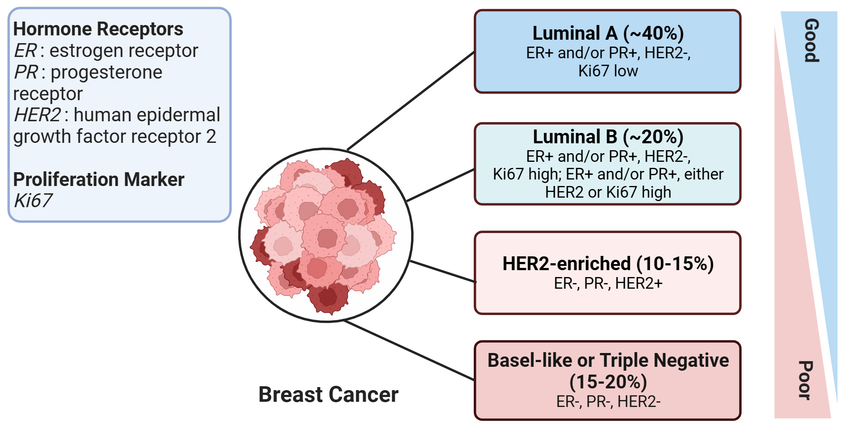
\includegraphics[width=0.8\linewidth]{reports/assets/subtypes.png}
    \caption{Resumen de los 4 subtipos moleculares del cáncer de mama y su porcentaje de relevancia \cite{harnessing_2024}}
    \label{fig:subtypes}
\end{figure}



\newpage

\section{Objetivos}

\begin{itemize}
  \item El objetivo principal es crear una herramienta que mediante mamografías pueda ser capaz de clasificar de manera eficiente entre los 4 subtipos moleculares, de forma que se pueda presentar como una alternativa viable a formas mucho mas invasivas y que pueden presentar muchos inconvenientes como las biopsias, u otros procedimeintos como los procesos Inmunohistoquímica (IHC) o Secuenciación Genética y Paneles Multigénicos (Oncotype DX, MammaPrint)
  \item Esto lo haremos enfocándonos en las arquitecturas de modelos de Computer Vision basados en Transformers (Visión Transformers), específicamente enfocados en la arquitectura MaxVit, debido a su mecanismo de atención local y global. Evaluaremos tambien los vision Transformers normales(ViTs) y los Swin Transformers, asi como tambien las arquitecturas mas tradicionales pero efectivas hasta el momento de CNN como puede ser ResNet101
  \item Evaluaremos métricas entre cada clasificador, alternando entre clasificación binaria, o multiclase, asi como tambien con fine-tunning o sin, para determinar que viene mejor en cada caso.
  \item Finalmente tambien, exploraremos la explicabilidad del modelo, esta parte es interesante por que nos permitiría una idea clara de que zonas podría estar relacionadas con cada clase. Para esto utilizaremos tecnicas como GradCAM, Saliency Maps o SHAP.
\end{itemize}

\begin{center}
  $\ast$~$\ast$~$\ast$
\end{center}


El objetivo principal de este estudio es desarrollar una herramienta basada en Inteligencia Artificial (AI), específicamente en aprendizaje profundo (Deep Learning, DL)\footnote{El Deep Learning es una rama del aprendizaje automático y la inteligencia artificial que se caracteriza por el uso de redes neuronales artificiales para el aprendizaje de patrones complejos.}, capaz de clasificar los cuatro subtipos moleculares del cáncer de mama a partir de imágenes mamográficas de pacientes diagnosticadas con esta enfermedad.

Para ello, se evaluará el desempeño de uno de los modelos más recientes de DL especializados en tareas de visión por computador, el Multi-Axis Vision Transformer (MaxVit). Este modelo, gracias a su mecanismo de atención tanto local como global y su capacidad para procesar imágenes de alta resolución, representa una alternativa prometedora para esta tarea.

Además, se realizará una comparativa del desempeño de MaxVit con modelos predecesores como Vision Transformer (ViT) y Swin Transformers (Shifted-Windows Transformers), así como con modelos basados en redes neuronales convolucionales, como ResNet-101.



\section{Cronograma}

%%%%%%%%%%%%%%%%%%%%%%%%%%%%%%%%%%%%%%%%%%%%%%%%%%%%%%%%%%%%%%%%%%%%%%%%%

\chapter{Background}

\section{Breast Cancer}


\begin{itemize}
  \item Definicición del cancer de mama
    \item Clasificación en subtipos moleculares
    \item Como se caracterizan estos subtipos
     \item Utilidades de estos subtipos
      \item Procedimientos estandar de clasificación (invasivos)
       \item Inteligencia artificial y deep learning
        \item IA en analisis de imagen
         \item IA como solucion
          \item Resultados anteriores
           \item Propuesta
            \item Transformers
             \item MaxVit
\end{itemize}


%%%%%%%%%%%%%%%%%%%%%%%%%%%%%%%%%%%%%%%%%%%%%%%%%%%%%%%%%%%%%%%%%%%%%%%%%
\backmatter
\selectlanguage{spanish}
\addcontentsline{toc}{chapter}{Bibliografía}
\bibliographystyle{ieeetr}
\bibliography{references}


\end{document}
